\documentclass[12pt]{article}
\usepackage[utf8]{inputenc}
\usepackage{geometry}
\geometry{
  a4paper,
  left=0.5in,
  right=0.5in,
  top=0.5in,
  bottom=0.5in
}
\usepackage{times}
\usepackage{setspace}
\onehalfspacing
\usepackage{graphicx}
\usepackage{pgfplots}
\pgfplotsset{compat=1.18}
\usepackage{amsmath}
\usepackage{booktabs}
\usepackage{parskip}
\usepackage{float} 
\usepackage[numbers]{natbib}
\usepackage{tocloft}
\setlength{\cftsecindent}{0pt}
\setlength{\cftsubsecindent}{0pt}
\usepackage{hyperref}
\hypersetup{
  colorlinks=true,
  linkcolor=blue,
  citecolor=blue,
  urlcolor=blue
}

% Ensuring Times New Roman equivalent
\renewcommand{\rmdefault}{ptm}

\begin{document}

% Title Page
\begin{titlepage}
  \centering
  \vspace*{1cm}
  {\LARGE\bfseries Effect of Foreign Films on the Moral Conduct of Undergraduate Students: An Exploratory Study at USTC, Bangladesh \par}
  \vspace{1cm}
{\large J.D. Milton\textsuperscript{1}, Mohammad hafizur Rahman Sakib\textsuperscript{2} \par}
\vspace{0.5cm}
{\normalsize
  \textsuperscript{1}Faculty, Department of English, Premier University,Chattogram \par
  \textsuperscript{2}Student, Department of Computer Science \& Engineering, Premier University,Chattogram \par
}
  \vspace{2cm}
\begin{abstract}
\fontsize{12.5pt}{15pt}\selectfont
This study explores the influence of foreign films on the moral and behavioral conduct of first-year undergraduate students in the Department of English at the University of Science and Technology Chittagong (USTC), Bangladesh. Using a mixed-method approach, data were collected from 20 students through a questionnaire with five quantitative multiple-choice questions and two qualitative opinion-based questions. Findings show high engagement with foreign films, particularly Hollywood (85\%) and Bollywood (65\%), with thrillers (50\%) and comedies (45\%) as top genres. Students are drawn to compelling stories (45\% first priority), themes, and characters, with 55\% viewing films as societal reflections. Benefits include cultural exposure and analytical skills, but risks involve moral desensitization, cultural erosion, and academic distraction. Recommendations advocate regulated viewing, media literacy, and a stronger local film industry to preserve Bangladeshi values. This research underscores the need for critical media consumption among youth.
\end{abstract}


  \vspace{0.5cm}
  {\normalsize \textbf{Keywords}: Foreign films, Moral conduct, Undergraduate students, Media influence, Cultural impact, Bangladesh, Thriller genre, Media literacy \par}
\end{titlepage}

% Table of Contents
\tableofcontents
\newpage

% Introduction
\section{Introduction}
Films are a powerful medium for storytelling, cultural exchange, and shaping societal values, influencing viewers’ moral and behavioral conduct through vivid narratives and imagery. In Bangladesh, the advent of streaming platforms like Netflix, YouTube, Amazon Prime, and Disney+ has made foreign films increasingly accessible, particularly to young audiences. This study focuses on first-year undergraduate students in the Department of English at the University of Science and Technology Chittagong (USTC), a private institution, to examine how foreign films impact their moral conduct, cultural perceptions, and academic engagement. The global reach of media has blurred cultural boundaries, introducing Western and Asian cinematic influences that may conflict with Bangladesh’s traditional and religious values. For example, exposure to violence, romanticized lifestyles, or explicit content in films can desensitize students or inspire behaviors misaligned with local norms. This exploratory research quantifies students’ film-watching habits, identifies preferred genres and film origins, and assesses their awareness of moral implications. By addressing these dynamics, the study contributes to the limited scholarship on media influence in Bangladesh’s tertiary education, advocating for media literacy and cultural preservation to balance global influences with local identity.

% Literature Review
\section{Literature Review}
The influence of media, particularly films, on youth behavior has been a subject of extensive research since the 1950s, when television emerged as a dominant entertainment form, reinforcing societal norms like patriotism and religious faith \cite{khan_academy_1950s}. The rise of streaming platforms has amplified this impact by providing instant access to global content \cite{pittman2015}. In South Asian contexts, including Bangladesh, this accessibility fosters cultural hybridity, often eroding indigenous values \cite{ndimele2004}. Research by \cite{riddle2017} indicates that 19\% of viewers engage in unintentional binge-watching, linked to addictive behaviors that impair academic performance. \cite{ali2019} suggests that foreign films highlight universal human experiences but reflect culturally specific responses, shaping viewers’ attitudes and coping mechanisms. \cite{muthu2021} notes that films compress intense emotions—love, hatred, violence—within hours, potentially desensitizing audiences to ethical concerns. \cite{aldana2004} underscores films’ conversational power to shape or disrupt cultural norms, while \cite{raji2020} links violent foreign films to aggressive youth behaviors. A study by \cite{johnson2016} on Nigerian youth found that Western media influences dressing (60.7\%), sexual conduct (60.5\%), and aggression, a trend relevant to Bangladesh, where students favor foreign films for their production quality \cite{brown2014}. \cite{meltzoff1977} associates heavy media exposure with societal aggression, emphasizing the need for selective viewing. In Bangladesh, the preference for Hollywood and Bollywood over local films risks cultural erosion, necessitating research into moral and behavioral impacts \cite{kubay1990}.

% Data Analysis
\section{Data Analysis}
This study employed a mixed-method approach to examine the impact of foreign films on 20 first-year undergraduate students (aged 18–21) in USTC’s Department of English. Data were gathered using a questionnaire with seven close-ended questions: five multiple-choice questions (MCQs) analyzed quantitatively and two opinion-based questions analyzed qualitatively. The MCQs included ranking questions (3 stars for first priority, 2 stars for second, 1 star for least) to assess film-watching frequency, preferred genres, film origins, and elements of fascination. Qualitative questions explored students’ views on films’ moral implications and their benefits and harms. Quantitative data were processed using percentages and visualized through charts, while qualitative responses were subjected to thematic analysis to identify patterns, such as concerns about violence or cultural incompatibility. The sample, though limited to 20 students, comprised engaged participants familiar with films, ensuring response authenticity. Limitations included the exclusion of faculty perspectives and the challenge of assessing moral awareness among students new to such critiques. The analysis correlated viewing habits with moral and behavioral changes, providing a structured overview of media consumption patterns.

% Findings
\section{Findings}
The study revealed detailed insights into students’ engagement with foreign films, supported by quantitative and qualitative data:

\begin{itemize}
  \item \textbf{Frequency of Watching}: 45\% of students watch films every 2–4 days, 15\% daily, 10\% weekly, 15\% occasionally, and 15\% rarely, indicating frequent media exposure.
  \item \textbf{Film Origins}: Hollywood films lead (45\% first priority, 85\% total engagement), followed by Bollywood (30\% first priority, 65\% total), and Korean films (5\% first priority, 50\% total). Tamilian (20\% total), Chinese/Japanese (20\% total), and Bangladeshi films (40\% total, no first priority) are less popular, reflecting a preference for foreign productions.
  \item \textbf{Genres}: Thrillers are most favored (50\% total, 30\% first priority), followed by comedy (45\% total), horror (35\% total), and action/romance (35\% each). Thrillers’ suspenseful plots and climactic narratives drive their appeal.
  \item \textbf{Fascinating Elements}: Students prioritize story/plots (45\% first priority), themes (30\% second priority), and characters (15\% first priority), influencing emotional and behavioral responses.
  \item \textbf{Perception of Reality}: 30\% believe films reflect societal realities, 25\% see them as depicting present and future possibilities, 25\% view them as unreal, and 20\% as somewhat real, indicating partial critical awareness.
  \item \textbf{Moral Concerns}: Students highlighted violence, sexual content, and culturally incompatible themes. One remarked, “No foreign movies can claim to be free from adultery content, but moral lessons are there.” Another criticized commercialized content: “Today’s foreign films focus on entertainment, showing violent and sexual content that misleads young minds.”
  \item \textbf{Benefits}: Exposure to diverse cultures, language learning, broadened perspectives, and analytical skills.
  \item \textbf{Harms}: Risks include conflating fiction with reality, trauma from disturbing scenes, cultural erosion, addiction, and reduced academic focus.
\end{itemize}

\begin{figure}[H]
\centering
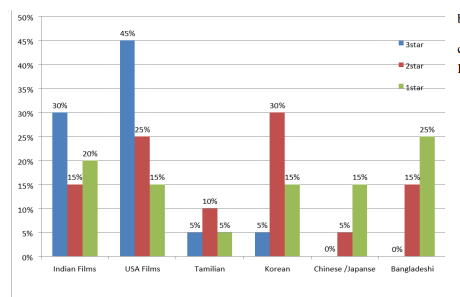
\includegraphics[width=0.9\textwidth]{1.png}
\caption{Frequency of Film-Watching Among Surveyed Students}
\label{fig:film_frequency}
\end{figure}

\begin{figure}[H]
\centering
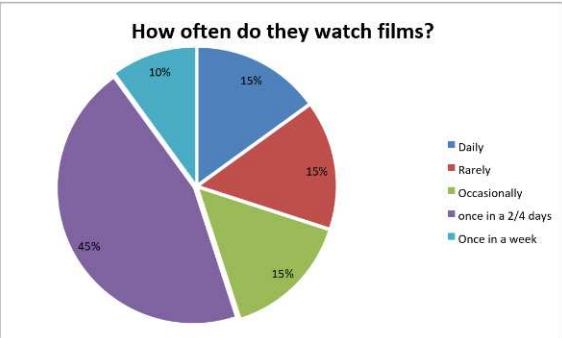
\includegraphics[width=0.9\textwidth]{2.png}
\caption{How often the surveyed students watch films?}
\label{fig:watching_frequency}
\end{figure}
\clearpage
% Results
\section{Results}
The findings confirm that foreign films significantly influence USTC students’ moral and behavioral conduct. High engagement with Hollywood (85\%) and Bollywood (65\%) films, particularly thrillers (50\%), shapes students’ perceptions, often normalizing violence or foreign cultural practices. For instance, 55\% view films as societal reflections, which may encourage emulating on-screen behaviors, such as aggressive or romanticized lifestyles, aligning with \cite{johnson2016} and \cite{meltzoff1977}. Benefits include cultural exposure and analytical skills, but these are overshadowed by risks like cultural erosion, as students overlook Bangladeshi films (0\% first priority). Addiction to binge-watching, evident in 15\% daily viewers, correlates with reduced academic focus \cite{riddle2017}. Commercialized content exacerbates moral desensitization, particularly when students lack critical awareness. Strengthening Bangladesh’s film industry could promote culturally relevant narratives, mitigating foreign influence and preserving local values.

% Conclusion
\section{Conclusion}
Foreign films profoundly impact the moral and behavioral conduct of first-year undergraduate students at USTC, presenting both opportunities and challenges. Benefits, such as cultural exposure, language acquisition, and analytical skill development, are significant, yet risks like moral desensitization, cultural erosion, and academic distraction are pressing concerns. Students’ partial awareness, with 55\% viewing films as societal reflections, highlights the need for enhanced media literacy to foster critical viewing. The dominance of Hollywood and Bollywood over local cinema underscores the urgency of revitalizing Bangladesh’s film industry to produce morally and culturally resonant content. Recommendations include limiting viewing to once weekly, prioritizing positive cultural elements, and avoiding blind imitation of foreign characters. Future research should involve larger, diverse samples, incorporating faculty and parental perspectives. By promoting selective viewing and cultural preservation, Bangladesh can balance global media consumption with the maintenance of students’ moral and cultural integrity.

% References
\section{References}
\bibliographystyle{plainnat}
\begin{thebibliography}{13}
\bibitem{ali2019}
Ali, F. (2019). Why foreign cinema can be better than Hollywood. \textit{Hello Student}. \url{https://www.hellostudent.co.uk/2019/04/why-foreign-cinema-can-be-better-than-hollywood/}

\bibitem{aldana2004}
Aldana, C. (2004). Can media regulation help in the search for equality? \textit{Media Development: Journal of the World Association for Christian Communication}, 51(4).

\bibitem{brown2014}
Brown, N. J., \& Bassey-Duke, V. (2014). Hollywood imperialism on Calabar-South teenagers. \textit{The Score Sheet}, 2, 11--25.

\bibitem{johnson2016}
Akintayo, J. B., \& Adegoke, A. (2017). Western entertainment television programmes: A catalyst for behavioural tendencies among students of Babcock and Covenant Universities. \url{https://www.academia.edu/33080765/Western_Entertainment_Television_Programmes_A_Catalyst_for_Behaviourial_Tendencies_among_Students_of_Babcock_and_Covenant_Universities}

\bibitem{khan_academy_1950s}
Khan Academy. (n.d.). Popular culture and mass media in the 1950s. \url{https://www.khanacademy.org/humanities/us-history/postwarera/1950s-america/a/popular-culture-and-mass-media-cnx}

\bibitem{kubay1990}
Kubay, R., \& Larson, R. (1990). The use of the experience of the new video media among children and young adolescents. \textit{Communication Research}, 17(1), 107--130.

\bibitem{larose2003}
LaRose, R., Lin, C. A., \& Eastin, M. S. (2003). Unregulated internet usage: Addiction, habit, or deficient self-regulation? \textit{Media Psychology}, 5(3), 225--253.

\bibitem{meltzoff1977}
Meltzoff, A. N., \& Moore, M. K. (1977). Imitation of facial and manual gestures by human neonates. \textit{Science}, 198(4312), 75--78.

\bibitem{muthu2021}
Muthu, V. K. (2021). Negative impact of cinema. \textit{Times of India Blog}. \url{https://timesofindia.indiatimes.com/readersblog/ezhil/negative-impact-of-cinema-30108/}

\bibitem{ndimele2004}
Ndimele, M. H. (2004). Globalizations and large languages as a threat to cultural and historical small Nigerian languages: The way forward. \textit{10th Annual Conference of ANLAT, Aba}.

\bibitem{nimcj2019}
NIMCJ. (2019). How mass media influence our society. \url{https://www.nimcj.org/blog-detail/how-mass-media-influence-our-society.html}

\bibitem{pittman2015}
Pittman, M., \& Sheehan, K. (2015). Streaming media and the new audience. \textit{Journal of Advertising Research}, 55(4), 345--356.

\bibitem{raji2020}
Raji, P. A. (2020). Perceived influence of foreign films on the behavioural pattern of teenagers in selected secondary schools in Ibadan, Oyo State. \textit{Chapter Two: The Consequences of Film}, 8.

\bibitem{riddle2017}
Riddle, K., Peebles, A., Davis, C., Xu, F., \& Schroeder, E. (2017). The addictive potential of television binge watching: Comparing intentional and unintentional binges. \textit{Journal of Behavioral Addictions}, 6(3), 37--48.
\end{thebibliography}

\end{document}